% --------------------------------------------------------------------

\section{Johdanto}

Nykyaikainen videodata tallennetaan digitaaliseen muotoon. Videodatan
käsittelyä digitaalisille tallennuslaitteille ja siirtokanaville sopivaan
muotoon ja uudelleen katseltavaan muotoon kutsutaan videokoodaukseksi.
Koodaaminen on tärkeää kaikenlaisen median, kuten äänen, kuvan ja videon,
digitaaliselle tallentamiselle. Videodatan erikoisominaisuus on se, että
se yhdistelee erilaisia medioita. Tämän seurauksena videodata vaatii suuren
määrän tallennustilaa ja siirtokapasiteettia, mikä tekee videon koodaamisesta
tärkeämpää. Samalla videodatan monialainen luonne lisää haasteita sen
kompaktiin esittämiseen. Olemassa olevia videokoodausmenetelmiä määräävät
standardi. (\citealt{h264})

Videodatan laadun kasvu ja tiedon langattoman siirtämisen yleistyminen pakottaa
kehittämään uusia, tehokkaampia videokoodausmenetelmiä. Ollaan kuitenkin tultu
siihen pisteeseen, että vain tehokkaimmat yksiprosessorijärjestelmät pystyvät
koodaamaan korkealaatuista videodataa. Kustannustehokkaan ja riittävän
laskentatehon saavuttamiseksi tarvitaan tulevaisuudessa muita ratkaisuja, kuin
ainainen yksittäisen prosessorin kellotaajuuden kasvatus (\citealt{moore}, \citealt{vajda}). Rinnakkaislaskenta
mahdollistaa halvemman ja paljon tehokkaamman ratkaisun laskentatehon
kasvattamiseen. (\citealt{xu}, \citealt{chi})

Videokoodaus on kuitenkin laskennallisesti jäykkä tehtävä videodatan runsaista
sisäisistä riippuvuuksista ja olemassa olevien videokoodausmenetelmien
toteutusten johdosta. Tästä johtuen videokoodausmentelmien rinnakkaistaminen ja
rinnakkaislaskennasta näkyvien hyötyjen saaminen on vaikeaa.
(\citealt{pieters}, \citealt{li}) Tämän työn tavoite on esitellä videokoodausta,
rinnakkaislaskentaa ja ratkaisuja rinnakkaisen videokoodauksen toteuttamiseksi.

Rinnakkaislaskennasta on tutkimusten mukaan hyötyä videokoodaukselle. Tärkeää
on ottaa rinnakkaislaskenta huomioon uusia standardeja suunniteltaessa, jotta ne leviävät
laajempaan käyttöön. Yleistyvät moniydeinprosessorit tukevat tätä ajatusta.
Jatkotutkimuksena kannattaisi tutkia, millaiset ratkaisut
soveltuvat mahdollisimman monelle rinnakkaiselle kiihdytysalustalle ja miten
mahdollisimman tehokkaita rinnakkaisia ratkaisuja olisi mahdollisimman helppo
tuottaa.

Luvussa \ref{chap:intro} käsitellään perusasioita elävästä kuvasta,
videokoodauksesta ja rinnakkaislaskennasta. Kappale toimii lyhyenä johdantona
työn aiheisiin, jos ne eivät ole aiemmin tuttuja.

Videodatan on luonteeltaan monijakoista, sillä se sisältää elävää kuvaa, ääntä
sekä mahdollisia lisäominaisuuksia. Videokoodauksen eri osat eivät ole
monimutkaisia operaatioita, mutta datan riippuvuudet ja sen määrä asettavat
haasteita videokoodausmenetelmille. Luvussa \ref{chap:coding} esitellään
videokoodauksen ja videodatan peruskäsitteitä sekä mittareita
videodatan ja videokoodauksen laadulle. Perinteiset videokoodausmenetelmät
käyttävät videodatan riippuvuuksia hyväkseen koodausprosessin parantamiseksi. (\citealt{h264}, \citealt{du})

Rinnakkaislaskennan tavoite on laskentatehon kasvatus monia laskentayksiköitä
hyödyntämällä. Rinnakkaisuuteen liittyy kuitenkin paljon haasteita, kuten laskennan
järjestäminen, sopivan rinnakkaisen toteutuksen löytäminen kulloinkin käsillä
olevaan ongelmaan ja suuri määrä erilaisia rinnakkaisia kiihdytysalustoja.
Luvussa \ref{chap:parallel} esitellään rinnakkaisuuden peruskäsitteitä,
haasteita ja  apoja mitata rinnakkaisten järjestelmien tehokkuutta.
Rinnakkaisten järjestelmien tehokkuuden mittamisessa tärkeintä on, että ne ovat
peräkkäisiä toteutuksia tehokkaampia. (\citealt{intro}, \citealt{rauber})

Rinnakkaislaskennan soveltaminen videokoodaukseen on erityisen hankalaa
videodatan riippuvuuksien ja datan määrän johdosta. Riippuvuuksien hyödyntäminen
on toiminut olemassa olevilla menetelmillä,
mutta videodatan laadun ja määrän kasvaessa nämä keinot alkavat olla
riittämättömiä ((\citealt{chi}, \citealt{xu})). Luvussa \ref{chap:parallel_coding}
esitellään rinnakkaisen videokoodauksen ongelmien lisäksi
luvussa joukko ratkaisuja sen toteuttamiseen. Ratkaisuja ovat uudet standardit, riippuvuuksien ja
synkronoinnin tarpeen vähentäminen ja mentelmien optimointi. Näillä keinoilla
on saavutettu näkyviä hyötyjä videokoodauksen tehokkuuteen ja laatuun.
(\citealt{pieters}, \citealt{chi}, \citealt{xu})

Työn johtopäätökset esitellän luvussa \ref{chap:conclusion}.



\begin{comment}
Sopivuudestaan huolimatta rinnakkaisohjelmointi ei kuitenkaan ole helppo
ratkaisu laskentatehon lisäämiseksi. Jotta rinnakkaisista järjestelmistä
saataisiin laskennallista hyötyä, täytyy laskenta järjestää huolellisesti.
Eri laskentayksiköiden välinen kommunikaatio, laskennan synkronointi ja
oikeellisuus ovat rinnakkaisohjelmoinnin suuria haasteita.
Rinnakkaisohjelmoinnin ongelma on myös se, että pitkään sillä saavutetut hyödyt
olivat pieniä verrattuna normaaliin laskentaan sen vaikeuksista johtuen. (\citealt{intro})
Toisaalta Mooren lain mukainen prosessoreiden tehon kasvu on tarkoittanut sitä,
että horisontissa on aina ollut tehokkaampia prosessoreita (\citealt{moore}). Nyt kuitenkin
alettu saavuttaa raja, jossa kaikkia yksittäiselle sirulle asetettuja
transistoreita ei voida käyttää esimerkiksi jäähdytyksen riittämättömyyden
johdosta. Rinnakkaiset ratkaisut ovat tulevaisuudessa välttämättömiä.

Rinnakkaisuuden omien ongelmien lisäksi videokoodaus tuo rinnakkaislaskentaan
omat haasteensa. Videodata on luonteeltaan moninaista ja sillä on runsaasti
sisäisiä riippuvuuksia. Lähes kaikki nykyiset videokoodausmenetelmät
hyödyntävät näitä riippuvuuksia koodausta nopeuttaakseen ja tallennustilaa
säästääkseen, mutta rinnakkaislaskennan kannalta nämä riippuvuudet vähentävät
rinnakkaistamisen mahdollistamista. Nykyisiä standardeja ei ole suunniteltu
rinnakkaisuutta silmällä pitäen. (\citealt{pieters}, \citealt{xu})

Videokoodauksen rinnakkaistaminen vaatii edellisissä kappaleissa esitettyjen
ongelmien ratkaisua, eivätkä ongelmat määrästään huolimatta ole mahdottomia.
Datan riippuvuuksia voidaan rikkoa, laskenta järjestää tehokkaaksi ja uusia
standardeita kirjoittaa. Rinnakkaislaskennalla on tuotu onnistuneesti lisätehoa
jo olemassa oleviin menetelmiin ja tulevien standardien suunnittelussa
rinnakkaisuus on jo otettu huomioon. (\citealt{li}, \citealt{chi})
Rinnakkaisohjelmointi tulee yleistymään kaikilla tietotekniikan
sovellusalueilla ja rinnakkaisohjelmointityökalut kehittymään. Vaikeuksista
huolimatta rinnakkaislaskenta on myös videokoodauksen tulevaisuutta.

Tämä työ keskittyy esittelemään ratkaisuja videokoodauksen rinnakkaistamiseen.
Lisäksi esitellään videokoodauksen ja rinnakkaislaskennan perusasioita, jotta
rinnakkaisen videokoodauksen hyödyt, tarpeellisuus ja haasteet tulisivat
esille. Aluksi esitellään digitaalisen liikkuvan kuvan peruskäsitteitä,
rinnakkaislaskennan historiaa ja joitakin näitä tukevia tieteenaloja. Tämän
jälkeen esitellään videokoodaus ja rinnakkaislaskenta. Lopulta esitellään
varsinaisia ratkaisuja rinnakkaiseen videokoodaukseen ja tehdään yhteenveto
tutkimuksen sisällöstä.
\end{comment}

\section{Digitaalinen liikkuva kuva ja rinnakkaislaskennan perusteet}
\label{chap:intro}

Tässä luvussa käsitellään digitaalista videota, rinnakkaislaskennan historiaa
sekä kahta liikkuvaan kuvaan ja rinnakkaislaskentaan liittyvää käsitettä,
havaitsemista ja rinnakkaislaskennan oikeellisuutta. Luvun tavoitteena on
toimia johdantona työn aiheisiin eikä niissä syvennytä mainittuihin teemoihin
kovin tarkasti.

\subsection{Digitaalinen video ja sen koodaus}

Ensimmäisistä liikkuvan kuvan sovelluksista 1800-luvun lopulta
alkaen elävä kuva on perustunut tallennettujen kuvanäytteiden nopeaan toistamiseen
liikkuvan kuvan vaikutelman aikaansaamiseksi.
Eräs ensimmäisistä ja pisimpään selvinneistä tallennusformaateista oli filmi,
jolle valotettiin peräkkäisiä valokuvia ja tulosta esitettiin projektorilla.
Vuosien saatossa tallennusmenetelmät ovat kehittyneet ja siirtomenetelmät
kehittyneet ensin analogisiksi radiosignaalien esimerkin innoittamana ja
myöhemmin digitaalisiksi digitaalisen vallankumouksen myötä. (\citealt{mitra})

Siirtymä digitaalisen videon aikakaudelle on tapahtunut viimeisen viidentoista
vuoden aikana. VHS-kaseteista ja analogisista TV-lähetyksistä
on siirrytty Blu-Ray -tekniikoihin, kännykkäkameroihin
teräväpiirtotelevisioihin. Tekniikan kehitys ei näy ainoastaan tallennusmedioissa,
vaan tiedonsiirtomenetelmät ovat niin ikään on kehittyneet ja muuttuneet monin paikoin
langattomaksi.(\citealt{h264})
Tallentamisen ja siirtämisen helpottumisen johdosta videodataa on maailmassa
yhä enemmän (\citealt{cisco}, \citealt{youtube}).

Raaka videodata vaatii suuret määrät tallennustilaa eikä sen siirtäminen
langattomasti ole mahdollista - tarvitaan siis teknologia, jolla videodataa pakataan ja puretaan
(enkoodataan ja dekoodataan). Tätä pakkaamisen ja purkamisen prosessia
kutsutaan videokoodaukseksi. Pakkaamisen ja purkamisen lisäksi videokoodaus kattaa
myös signaalin reaaliaikaisesta kääntämisestä (transkoodaus). Transkoodaus
tarkoittaa esimerkiksi enkoodatun datan kääntämistä toiseen koodausstandardiin (\citealt{mpeg_app}).
Koodekki (CODEC, lyhenne sanaparista coder decoder pair) on videokoodausta suorittavaan
ohjelmisto tai laite (\citealt{h264}). Videokoodausta käsitellään luvussa \ref{chap:coding}.

Videokoodausstandardeja on useita, mainittakoon tässä H.264, MPEG-4 ja DICOM,
joista kaksi ensimmäistä ovat kuluttajakäyttöön suunniteltuja standardeja
ja viimeinen lääketieteelliseen kuvantamiseen suunniteltu. (\citealt{h264})

\subsection{Rinnakkaislaskennan perusteita}

Rinnakkaislaskennan (parallel computing) tavoite on parantaa laskennan
suorituskykyä. Käsitteellisesti rinnakkaislaskentaa ei kannata sekoittaa
samanaikaiseen laskentaan (concurrent computing). Akateemisessa mielessä
jälkimmäinen keskittyy rinnakkaisen laskennan oikeellisuuteen, kun taas
ensimmäinen keskittyy saamaan hajautetusta ja rinnakkaisesta laskennasta
näkyviä hyötyjä laskentatehoon. (\citealt{intro}, \citealt{ari}) Tämä työ keskittyy
rinnakkaisella laskennalla saavutettuihin hyötyihin videokoodauksen saralla,
mutta myöhemmin tässä luvussa esitellään lyhyesti rinnakkaislaskennan
oikeellisuuden tarkastelua.

Rinnakkaislaskennan nimi on suuntaa-antava. Laskennan suorituskykyä pyritään parantamaan
suorittamalla laskentaa mahdollisimman monella laskentayksiköllä samaan aikaan.
Ajatus on looginen - jos yhdeltä laskentayksiköltä kestää yhden aikayksikön
suorittaa jokin laskentatehtävä, niin sadan laskentayksikön suorittaminen
kestää sata aikayksikköä. Sadalta laskentayksiköltä taas menee samaan tehtävään
vain yksi aikayksikkö. Intuitiivisesta perusajatuksesta huolimatta
rinnakkaislaskennalla on mittavat ongelmat, joiden
johdosta se on pysynyt kehityksen marginaalissa vuosikymmeniä.
(\citealt{intro}) Näihin ongelmiin ja rinnakkaislaskennan muihib piirteisiin
keskitytään rinnakkaislaskentaa käsittelevässä luvussa \ref{chap:parallel}.

\subsection{Rinnakkaislaskennan oikeellisuus}
\label{sec:model}

Laskentatehon lisäyksen lisäksi rinnakkaisuus lisää virhelähteitä laskentaan.
Monen laskentayksikön samanaikainen muistinkäsittely, laskennan aikataulutus ja viestikanavien käyttö ovat
esimerkkejä virheläheistä, joita ei perinteisessä peräkkäisessä ohjelmoinnissa
esiinny. Rinnakkaisten järjestelmien oikeellisuuden tarkastelua vaikeuttaa se,
että virheitä on vaikea toistaa. Virheet saattavat riippua hyvin tarkoista
ajoituksista ja sopivista suoritusjärjestyksistä ohjelman ajon aikana eivätkä
täten toistu kaikkien ajojen aikana. (\citealt{ari})

Yrityksellä ja erehdyksellä virheiden etsiminen on kallista ja aikaa vievää,
joten parempia keinoja tarvitaan. Eräs analyyttinen ratkaisu
rinnakkaislaskennan oikeellisuuden tarkasteluun on mallintarkistus. Tässä
menetelmässä rinnakkainen ohjelma kuvataan mallina, joka täyttää jollekin
abstraktion tasolle asti ohjelmalle asetetut vaatimukset. Mallia voidaan
tutkia automaattisilla työkaluilla, jotka paljastavat mahdollisia
rinnakkaisuuden ongelmia, kuten muistin ylikirjoittamista, ei-toivottuja
kisatilanteita tai laskennan umpikujia (deadlock). (\citealt{ari})
Mallintarkastus on laskennallisesti erittäin vaativa tehtävä, mutta se saattaa
säästää järjestelmän myöhemmiltä, mahdollisesti hyvin kalliilta ja vaikeilta
ongelmilta.

Tässä työssä ei tarkemmin syvennytä rinnakkaislaskennan oikeellisuuteen, mutta
se on eräs rinnakkaislaskennan monista ongelmista ja aktiivisen tutkimustyön kohde.

\section{Videokoodaus}
\label{chap:coding}

Tässä luvussa käsitellään videokoodauksen perusteita. Luvun tavoite on
antaa riittävät taustatiedot videokoodausmenetelmistä, jotta myöhemmässä
vaiheessa tätä työtä voidaan esitellä rinnakkaisia
videokoodausmenetelmiä sekä antaa hyvä yleiskuva videokoodauksesta. Yleisen
käsittelyn lisäksi tekstissä on esitelty lyhyesti muutama mielenkiintoinen
tutkimus, jotka ratkovat joitakin videokoodauksen ongelmia.

\subsection{Videokoodauksen peruskäsitteet}

\subsubsection{Videokuvan esittäminen ja tallentaminen}

Havaitsemamme maailma on täynnä erilaisia kohteita, joilla on
erilaisia ominaisuuksia, kuten muoto, syvyys, tekstuuri, väri tai valotiheys.
Maailma on niin ikään jatkuva, mitä esimerkiksi digitaalinen maailma ei ole. Jotta kameralla tai vastaavalla
laitteella voitaisiin tallentaa esitys maailmasta, täytyy havainnot käsitellä ja
tallentaa digitaaliseen maailmaan sopivaksi.

Videodataa varten maailmasta täytyy kerätä näytteitä eri ajanhetkiltä. Otanta
tapahtuu kahdessa ulottuvuudessa, ajassa ja tilassa (temporal and spatial
sampling). Tyypillisesti tilaotokset ovat suorakaiteen muotoisia kuvia
maailmasta, kun ajallinen otanta koostuu peräkkäisistä tilaotoksista.
Tilaotokset koostuvat neliönmuotoisista kuvapisteistä eli pikseleistä, jotka
on järjestetty ruudukoksi. Käsittelemättömättömiä aika- ja
tilanäytteitä kutsutaan raakadataksi. (\citealt{h264}, \citealt{du})

Jokaisen tilanäytteen kuvapisteeseen tallennetaan pisteeseen liittyvät
tiedot. Yksinkertaisinta kuvaa eli mustavalkokuvaa varten riittää
tallentaa vain yksi arvo kuvapisteestä (kirkkaus tai valotiheys), mutta
värikuvassa täytyy tallentaa jokaisessa pisteessä esiintyvien värien määrä.
Väriavaruudeksi kutsutaan menetelmää, joka on valittu kuvapisteiden kirkkauden,
valotiheyden ja värin kuvaamiseksi. Värikuvan tallentamisessa suosittu tapa on
RGB-väriavaruus. Tässä menetelmässä jokaisella kuvapisteellä on
kolme parametria: punaisen, vihreän ja sinisen värin määrä. RGB-väriavaruudessa 
valotiheys ja väri ovat samanarvoisia, mutta edistyneemmät
väriavaruudet hyödyntävät ihmisaivojen suurempaa herkkyyttä valotiheydelle
kuin väreille. (\citealt{h264}, \citealt{du}) Väriavaruudet ovat matemaattisia
malleja havaitusta maailmasta. Niille on paljon erilaisia implementaatioita,
joihin ei tämän työn puitteissa syvennytä tarkemmin.

Avaruudellisia näytteitä voidaan ottaa joko peräkkäin (progressive) tai
lomittain (interlacing). Peräkkäisessä otannassa jokaisella ajanhetkellä
otetaan otos, johon tallennetaan käytössä olevan standardin mukainen
määrä kuvapisteitä. Otosta kutsutaan ruuduksi (frame). Lomittaisessa
otannassa taas jokaisella ajanhetkellä tallennetaan puolet standardin
määräämistä kuvapisteistä vaakasuunnassa joka toinen rivi siten, että
peräkkäisillä ajanhetkillä tallennetaan lomittaiset rivit. Otosta kutsutaan
kentäksi (field). Erotuksena näillä metodeilla on siinä, että lomittaisella
otannalla syntyy pehmeämmin liikkuvaa kuvaa kuin peräkkäisellä otosten määrän
ollessa sama. Lomittamalla jokaiseen otokseen tallennetaan myös vähemmän tietoa.
(\citealt{h264}, \citealt{du})

\subsubsection{Videodatan muut osat ja synkronointi}

Videodata ei koostu ainoastaan varsinaisesta videokuvasta, vaan kuvan lisäksi
tallennusvaiheessa tallennetaan ääntä. Ääniraita enkoodataan kuvadatan tavoin
halutulla menetelmällä ja tallennetaan kuvadatan oheen. Tässä
työssä ei syvennytä tarkemmin äänen koodaamiseen, mutta perusperiaatteet
pakkausmenetelmissä ovat samankaltaiset. Kuvan ja äänen lisäksi videokoodauksen
eri vaiheissa dataan voidaan lisätä haluttuja ominaisuuksia, kuten tekstitystä.
Lisäominaisuudet tallennetaan usein varsinaisesta videodatasta erillään. (\citealt{mpeg_app},
\citealt{mujal})
 
Videodatan osien ollessa erillisiä tarvitaan keino tahdistaa data eri
lähteistä hyvän katselukokemuksen takaamiseksi. Perusmenetelmiä on kolme.
Ensimmäinen on aikaleimatahdistus (Time-Stamps Synchronization), jossa eri
lähteisiin lisätään aikaleimoja. Aikaleimojen perusteella osataan eri lähteistä
tuleva data näyttää käyttäjälle samanaikaisesti. Toinen keino on
tahdistusmerkki (Synchronization Marker), joka käytännössä tarkoittaa eri datalähteiden välistä
kommunikaatiota, käytännössä merkin lähettämistä ja vastaanottamista, tahdistuksen
saavuttamiseksi. Kolmas on limitystahdistus (Multiplex Synchronization), jossa
limitetään eri datalähteet yhdeksi lähteeksi hyödyntäen näin niiden
luonnollista järjestystä tahdistuksen saavuttamiseksi. (\citealt{sync}, \citealt{mujal})

Perusmenetelmien lisäksi on tutkittu erilaisia metodeita
sulauttaa ääntä ja lisäominaisuuksia varsinaiseen videodataan pakkauksen tehostamiseksi
ja synkronoinnin vähentämiseksi.
Tällöin enkoodausvaiheessa kuvadataan lisätään äänidataa tai tiedot lisäominaisuuksista.
Tiedon sulauttamista kutsutaan joissain tutkimuksssa tiedon piilottamiseksi.
Tehdyssä tutkimuksessa videon tai kuvan laadun heikkeneminen ei ollut ihmissilmällä
havaittavissa. (\citealt{sync}, \citealt{mujal}, \citealt{hiding})

\subsubsection{Pakkaus ja ennustaminen}

Kaikenlaisen median pakkausmetodit voidaan jakaa häviöttömiin
ja häviöllisiin pakkausmetodeihin (lossy, lossless). Häviöttömissä metodeissa pakatusta datasta
pystytään purkuvaiheessa palauttamaan täydellinen versio alkuperäisestä
datasta, häviöllisessä pakkauksessa purettu versio on approksimaatio
alkuperäisestä. On olemassa häviöttömiä videokoodausmenetelmiä, mutta
pakkaussuhde jää liian alhaiseksi käytännön sovelluksiin. Häviölliset
pakkausmenetelmät keskittyvät poistamaan datasta subjektiivista redundanssia
eli yksityiskohtia, jota havainnoija ei kykene havaitsemaan. Näin
saavutetaan huomattavasti tehokkaampia videokoodausmenetelmiä. (\citealt{h264}, \citealt{du})
Toisaalta esimerkiksi lääketieteelliset sovellukset tai konenäkösovellukset
vaativat korkealaatuista kuvaa, jolloin häviötön pakkaaminen on ainoa
vaihtoehto (\citealt{xu}).

Suurin osa videokoodausmenetelmistä hyödyntää videodatan vahvaa
avaruudellista ja ajallista redundanssia. Käytännössä peräkkäisissä
ruuduissa on suurella todennäköisyydellä lähes samat kuvapisteet (ajallinen) ja
yhdessä ruudussa lähekkäiset kuvapisteet muistuttavat toisiaan suurella
todennäköisyydellä (tilallinen). Monien koodekkien ensimmäinen askel videon koodaamiseen
on ennustaminen - jollakin määrällä edellisiä ajallisia näytteitä voidaan
melko suurella todennäköisyydellä ennustaa, mitä tässä näytteessä tulee
olemaan. Samaan tapaan saman näytteen sisällä jo käsiteltyjen kuvapisteiden
perusteella ennustetaan tulevien kuvapisteiden laatua. Ennustuksilla voidaan
vähentää tallennettavan datan määrää, kun purkuvaiheessa näytteitä pystytään
uudelleenrakentamaan edellisten näytteiden perusteella. Läheisesti
ennustamiseen liittyvä käsite on liikekompensaatio (motion compensation).
Käytännössä liikekompensaatio on ennustamisen apukeino. Liikekompensaation
johdosta ei verrata
ainoastaan peräkkäisissä näytteissä samoilla koordinaateilla
olevia kuvapisteitä vaan myös sopivalla tavalla lähialueilta valittuja
pisteitä. (\citealt{h264}, \citealt{du})

\subsection{Videodatan riippuvuudet}
\label{sec:depend}

Videodata on luonteeltaan monijakoista sen sisältäessä niin liikkuvaa kuvaa,
ääntä kuin mahdollisia lisäominaisuuksia. Näiden sekä
enkoodauksen aikaisen ennustamisen johdosta koodatulla videodatalla on vahvoja
riippuvuussuhteita. Riippuvuuksia on kahdentyyppisiä. Ajallinen riippuvuus
tarkoittaa tässä yhteydessä sitä, että onnistunut videodatan
toistaminen on riippuvainen kaikista videodatan osien samanaikaisesta
toistamisesta. Datariippuvuutta syntyy ruutujen ja kenttien
sisällä esimerkiksi ennustettaessa uuden kuvapisteen arvoa edellisten
kuvapisteiden perusteella tai uusia näytteitä ennustettaessa  vanhojen
perusteella. (\citealt{mujal})

\begin{comment}
Riippuvuudet vaikeuttavat videokoodausprosessia ja lisäävät siihen ylimääräisiä
synkronointia ja monimutkaisuutta verrattuna esimerkiksi pelkän äänen koodamiseen.
Seuraavassa aliluvussa käsiteltävä diskreetti kosinimuunnos ja muut koodaukseen
liittyvät operaatiot eivät ole itsessään kovin vaativia, mutta koodekit ovat
kuitenkin varsin suuria ohjelmistoja kaiken laskentaa tehostavien lisäysten
johdosta. Esimerkiksi x264-ohjelmisto, joka on avoimen lähdekoodin toteutus
suositusta H 264 -standardista (\citealt{h264}), on n. 100 000 riviä koodia (\citealt{x264}).
\end{comment}

Riippuvuuksien johdosta videokoodausprosessi on laskennallisesti jäykkä, mikä
vaikeuttaa videokoodausmenetelmien rinnakkaistamista. Näitä ongelmia
käsitellään tarkemmin luvussa \ref{sec:problems}. Videokoodauksen yksittäiset
vaiheet eivät ole monumutkaisia, mutta synkronoinnin ja erilaisten laskentaa
tehostavien optimointin johdosta koodekit ovat varsin suuri ohjelmistoja. Esimerkiksi
Esimerkiksi x264-ohjelmisto, joka on avoimen lähdekoodin toteutus
suositusta H 264 -standardista (\citealt{h264}), on n. 100 000 riviä koodia (\citealt{x264}).

Rinnakkaislaskennan lisäksi on ehdotettu luoviakin ratkaisuja videokoodauksen
tehostamiseksi. \citealt{lee} ehdottaa menetelmää, jossa videon
äänilähteet piirretään suuremmalla tarkkuudella, koska ihmisten on luonteva
keskittää huomionsa äänilähteisiin. Mainitut lähteet (\citealt{mujal},
\citealt{sync}) esittelevät keinoja helpottaa videodatan synkronointia ja vähentää
tallennustilan tarvetta.

\subsection{Diskreetti kosinimuunnos}

Ennen tallentamista tai siirtämistä videodataa useimmiten käsitellään vielä
jollain tavalla ennustusten lisäksi. Tavoitteena on vähentää tallentamiseen
tarvittavaa muistia ja helpottaa aikanaan tapahtuvaa dekoodausta. Tekniikoita
on monia, mutta esitellään tässä tunnetuin, eli diskreetti kosinimuunnos
(Discrete Cosine Transformation, DCT). 

DCT on Fourier-muunnoksen kaltainen muunnos, joka operoi $N \times N$
kokoisilla blokeilla avaruudellisissa näytteissä. Muunnos tuottaa niin
ikään $N \times N$ kokoisen blokin, mutta kuvapisteiden arvojen sijaan
uuden blokin arvot ovat kosinimuunnoksen peruslohkojen suhteellisia
voimakkuuksia koodattavassa olevassa lohkoissa. Kuvassa \ref{fig:dct} on esitetty
$8  \times 8$ -lohkon DCT:n peruslohkot. (\citealt{h264})

\begin{figure}[ht]
	\centering
	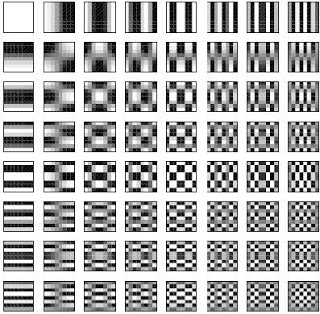
\includegraphics[width=0.5\textwidth]{dct.jpg}
	\caption{$8 \times 8$ DCT:n peruslohkot}
	\label{fig:dct}
\end{figure}

DCT:n hyöty ei ole ilmeinen, sillä muunnos tapahtuu $N \times N$ -lohkosta
$N \times N$ -lohkoon, eikä tässä säästetä lainkaan  tilaa. Hyöty ilmenee
purkuvaiheessa - on mahdollista purkaa DCT:n avulla tallennettua tietoa
riittävän tarkaksi käyttämällä vain osaa DCT:n tuottamista suhteellisista
voimakkuuksista. Voidaan siis tallentaa vain osa DCT:n tuottamista arvoista
ja käyttää näin vähemmän tilaa tiedon tallentamiseen. Tyypillisesti käytetään
DCT:n tuottamat suurimmat arvot eli merkityksellisimmät peruslohkot, jolloin
harvinaisemmat ja räikeimmät erot jäävät puuttumaan lopullisesta kuvasta.
Piirtämättä jäävät sellaiset yksityiskohdat, joita ihmissilmä on muutenkin
heikko havaitsemaan. DCT:tä käyttävät koodausmenetelmät ovat siis pääosin
häviöllisiä. (\citealt{h264}, \citealt{du})

\subsection{Videodatan matka lähteestä näyttölaitteelle}

Videodata saa alkunsa lähteestä, joka on tyypillisesti kamera, joka tallentaa
raakadatan. Tämän jälkeen suoritetaan koodekki suorittaa enkoodauksen, minkä
jälkeen tiivistetty data voidaan tallentaa tai siirtää. Ketjun toisessa
päässä on jälleen koodekki joka suorittaa tällä kertaa dekoodauksen ja esittää
videon käyttäjälle. Kuva \ref{fig:codec} havainnollistaa videodatan eri reittejä
käyttäjälle. (\citealt{h264})

\begin{figure}[ht]
	\centering
	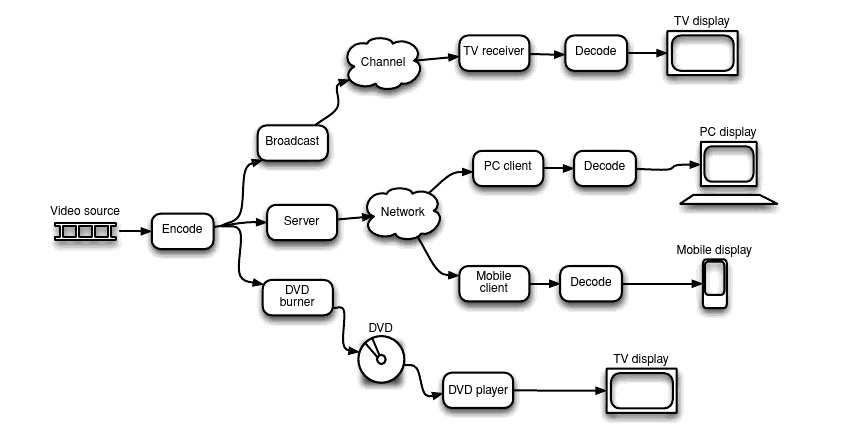
\includegraphics[width=0.8\textwidth]{codec.jpg}
	\caption{Videokoodaus mahdollistaa datan liikkuvuuden}
	\label{fig:codec}
\end{figure}

Koodauksen kolmas muoto, transkoodaus, tulisi tehdä, jos haluttu näyttölaite ei
tuekaan sille tarjottua koodaustapaa.

\subsection{Kuvadatan ja videokoodauksen laadun mittarit}
\label{sec:quality}

Videodatan laatua voidaan mitata subjektiivisesti ja objektiivisesti.
subjektiivinen mittaaminen on vaikeaa, sillä ihmisten arvioihin vaikuttavat
monet seikat. Objektiivinen mittaaminen taas antaa selviä lukuja vastaukseksi,
mutta tulosten merkitys ja vaikutus katsojakokemukseen on selvitettävä erikseen.
Videodatan kohdalla subjektiivista mittaamista voidaan usein pitää tärkeämpänä
kuin objektiivista, sillä tavoitteena usein on mahdollisimman miellyttävän
katselukokemuksen tuottaminen käyttäjälle. (\citealt{h264}) Toisaalta videodatan objektiivinen
laatu on erityistapauksissa myös tärkeää, esimerkiksi konenäköä hyödyntävissä
sovelluksissa tai koneiden muuten tulkitessa videodataa. Videodatan määrän
kasvaessa jatkuvasti ja konenäkösovellusten, kuten robottien, lisääntyessä
saattaa objektiivisesta laadusta tulla subjektiivista tärkeämpää (\citealt{youtube},
\citealt{cisco}).

Subjektiivinen laadun mittaamiseen liittyy olennaisesti havaitseminen.
Subjektiivista laatua voidaan mitata esimerkiksi kyselytutkimuksilla ja
havaitsemistutkimyksen muita keinoja, kuten silmänliikeanalyysiä, voidaan
käyttää videokoodausmenetelmien arvioimiseen ja kehittämiseen. (\citealt{perception})

Seuraavassa esitellään muutamia objektiivisia tapoja mitata videodatan laatua.

Tiheys, jolla ruutuja tallennetaan, määrää ruutunopeuden (frame rate).
Ruutunopeus ja kuvapisteiden määrä tarjoaa helpon mittarin kuvan laadulle.
Normaalitarkkuuksinen ja korkeatarkkuuksinen (Standard Definition, High
Definition) videodata eroavat toisistaan juuri kuvapisteiden määrän ja
ruutunopeuden perusteella. Valittu ruutujen tai kenttien esitystapa vaikuttaa
kuitenkin subjektiiviseen laatuun, joten ruutunopeuden ja kuvapisteiden määrää
ei voi pitää ehdottomana laadun mittarina. (\citealt{h264}, \citealt{du})

Yleisesti käytetty mittari videodatan laadun mittaamiseen on PSNR-arvo (Peak
Signal to Noise Ratio). PSNR kertoo erosta alkuperäisen ja uuden kuvan välillä
ja se on määritelty

\begin{center}
\begin{equation}PSNR_{dB} = 10\log_{10}\frac{(2^n - 1)^2}{MSE},\end{equation}
\end{center}

missä MSE on keskimääräinen neliöity virhe (Mean Squared Error) alkuperäisen 
kuvan ja uuden kuvan välillä. (\citealt{h264})

PSNR on helppo laskea ja antaa erään objektiivisen arvion videon laadusta.
Menetelmällä on puutteensa, kuten se, että alkuperäistä kuvaa ei ole
välttämättä saatavilla. Toisaalta, kuten monissa objektiivissa mittareissa,
pelkkä PSNR arvo ei vastaa suoraan mitään subjektiivista arvoa. Yleisesti
ottaen korkea PSNR arvo tarkoittaa hyvää laatua ja matala arvo huonoa.
(\citealt{h264}, \citealt{du})

Videokoodauksen laatua voidaan mitata esimerkiksi koodausnopeudella tai
pakkaussuhteella, eli raakadatan ja pakatun datan koon suhteella. (\citealt{li},
\citealt{xu}). Koodausnopeuden yksikkönä voidaan pitää esimerkiksi
$frac{ruutua}{sekunti}$.

\section{Rinnakkaislaskenta}
\label{chap:parallel}

Tässä luvussa käsitellään rinnakkaislaskennan perusteita ja haasteita.
Tekstissä esitellään lyhyesti
myös kuuluisa Amdahlin laki sekä muutama tutkimus automaattisten
rinnakkaistamisen toteutukseen.

\subsection{Rinnakkaisuus tietokonejärjestelmissä}

Rinnakkaisuutta esiintyy tietokonejärjestelmissä monessa muodossa.
Nykyaikaisissa supertietokoneissa on jopa yli miljoona ydintä (\citealt{top500}).
Toisaalta suurten supertietokoneiden lisäksi rinnakkaisuus on tullut aivan tavallisten
kuluttajatietokoneiden osaksi moniydinprosessoreiden myötä. Prosessorit ovat jo pitkään hyödyntäneet
erilaisten laskentayksiköiden samanaikaista käyttöä laskennan tehostamiseen.
Viimeksi mainittu menetelmä tunnetaan termillä liukuhihnaus (pipelining).
Liukuhihnalaskennan tehonlisäys seuraa siitä, että laskentaa voidaan
prosessorissa suorittaa suuremmalla kellotaajudella rinnakkaisten operaatioiden
johdosta. Samalla rinnakkaisuutta esiintyy kerroksittain, esimerkiksi
tavallisessa moniydinprosessorissa on monta ydintä, ja jokaisella ytimellä on
omat liukuhihnansa. (\citealt{intro}, \citealt{rauber})

\subsection{Rinnakkaisten menetelmien hallintarakenteet}

Rinnakkaislaskennan hallintarakenteet voidaan jakaa karkeasti kahteen luokkaan sen perusteella,
miten paljon laskennan hallintaa kullekin laskentayksikölle on jaettu. Jos
hallinta on keskitetty, kyseessä on SIMD-arkkitehtuuri (Single Instruction
stream, Multiple Data stream). SIMD-arkkitehtuurissa yksittäinen
hallintayksikkö päättää, mitä kukin laskentayksikkö laskee.
MIMD-arkkitehtuurissa (Multiple Instrucrion stream, Multiple Data stream)
jokaisella laskentayksiköllä on oma hallintayksikkönsä. Konkreettisena
esimerkkinä arkkitehtuurien erona voi pitää esimerkiksi sitä, että
MIMD-arkkitehtuurissa jokainen laskentayksikkö voi suorittaa eri ohjelmia, kun
SIMD-arkkitehtuurissa hallintayksikkö päättää, mitä ohjelmaa kaikki
laskentayksiköt suorittavat. Laskennan pilkkomista ja jakamista
laskentayksiköille SIMD-menetelmässä kutsutaan vektoroinniksi. (\citealt{intro}, \citealt{rauber})

Rinnakkaiset järjestelmät voidaan jakaa myös manycore- ja
multicore-järjestelmiin \footnote{Suomen kielessä sana moniydinprosessori
vittaa tyypillisesti multicore-järjestelmään}. Yhteistä molemmille
järjestelmille on useat laskentayksiköt. Multicore-järjestelmässä eri
ydinten välimuistit on pakotettu yhtenäiseen tilaan. Toisin sanoen yhden
ytimen laskennan tulokset päivitetään kaikkien muiden ytimien välimuisteihin.
Manycore-järjestelmissä välimuistien yhtenäisyysvaatimukset eivät ole yhtä
tiukkoja, joten manycore-järjestelmiä voidaan tässä mielessä pitää
multicore-järjestelmiä rinnakkaisempina. (\citealt{vajda})

\subsection{Rinnakkaisuuden peruskäsitteitä}

Hallintarkanteiden ja eri tasojen rinnakkaisuuksien lisäksi rinnakkaisuus voidaan jakaa
kahteen tyyppiin sen perusteella, mihin rinnakkaisuus kohdistuu.
Tehtävärinnakkaisessa laskennassa rinnakkain suoritetaan erilaisia
tehtäviä - esimerkiksi saman ohjelman eri säikeitä. Datarinnakkaisessa
ohjelmoinnissa taas rinnakkaisuus syntyy siitä, että operoidaan samaan aikaan
datan eri osa-alueilla. (\citealt{intro})

\subsubsection{Tiedon välittäminen laskentayksiköiden välillä}

Rinnakkaisuuden kohteen lisäksi rinnakkaisilla kohteilla on erilaisia tapoja
järjestää tiedon liikkuminen laskentayksiköiden välillä. Pääparadigmoja on
kaksi, jaettu muisti (shared memory) ja viestinvälitys (Message Passing Interface, MPI). Jaetun muistin mallissa
laskentayksiköillä on yhteinen muisti, josta jokainen saa lukea ja kirjoittaa.
Jotta yhteinen muisti pysyy puhtaana eli kaksi laskentayksikköä ei lue ja/tai
kirjoita samaan muistiosoitteeseen samaan aikaan, täytyy järjestelmällä
olla keinot päättää milloin mitäkin muistialuetta saa käsitellä.
Erilaisia ratkaisuja tähän poissulkevuuden ongelmaan (mutual exclusion) on useita, kuten
monitorit tai semaforit. Samojen muistialueiden käsittelyyn
liittyy myös käsite kisatilanteista (race condition). Kisatilanteessa kaksi
laskentayksikköä tavoittelee samaa muistialuetta, mutta valitun
muistinsuojausmenetelmän pitäisi estää tämä. Kisatilanteet eivät varsinaisesti
ole rinnakkaisten ohjelmien vikoja vaan syntyvät rinnakkaisohjelmoinnin
sivutuotteena. (\citealt{ari})

Viestinvälitysmenetelmässä jokaisella
laskentayksiköllä on oma muistiavaruutensa, ja jos esimerkiksi  yksiköiden
välillä halutaan synkronoida, niin ne vaihtavat viestejä. Menetelmä vaatii,
että jokaisella laskentayksiköllä on tunniste, jolla sen voi erottaa muista.
Tämä vaatimus ei koske jaetun muistin menetelmää. Luonnollisesti viestien
välittämiseen tarvitaan myös jokin kanava niiden toimittamiseen. Viestien
välittäminen on jaetun muistin käyttämistä tehottomampaa, mutta sitä
käyttämällä on helpompi pitää yllä erilaisia laskentayksiköitä. Kaikkien
käyttäessä samaa muistia yksiköiden tulee käsitellä muistia samalla tavalla,
mutta viestejä välittäessä jokaisen yksikön täytyy vain täyttä
viestinvälitysrajapinnan vaatimukset. (\citealt{intro}, \citealt{rauber})

\subsubsection{Skaalautuvuus}

Skaalautuvuus kertoo saavutetaanko rinnakkaislaskennasta laskentayksiköiden määrään
suhteessa olevaa hyötyä, eli tehostuuko laskenta laskentayksiköitä lisäämällä.
Laskentayksiköiden lisääminen ei loputtomasti kasvata rinnakkaislaskennan
tehokkuutta. Hyvin skaalautuvan rinnakkaislaskentamallin laskenta-aika pysyy
vakiona ongelmaa ja laskentayksiköiden määrää kasvattaessa. (\citealt{rauber})
Toinen hyvin skaalautuvan rinnakkaisen ratkaisun merkki on, että sen suorityskyky
kasvaa lineaarisesti laskentayksiköiden määrää kasvatettaessa (\citealt{intro}).
Skaalautuvuus on välttämätön vaatimus tehokkaille rinnakkaisille järjestelmille
(\citealt{intro}. \citealt{rauber}).

\subsubsection{Rakeisuus ja laskennan järjestäminen}

Jotta laskentatehtäviä voidaan suorittaa rinnakkaisesti, täytyy tehtävät
hajottaa (decompose) pienempiin osiin. Hajotusta tehdessä otetaan huomioon laskennan
erilaiset riippuvuudet ja jaetaan laskentatehtävä pienempiin osatehtäviin.
Tiedot riippuvuuksista täytyy tallentaa myöhempää käsittelyä varten.
Kaikki osatehtävät eivät välttämättä ole samankokoisia ja kun jako on tehty,
kukin osatehtävä on uusi, jakamaton laskennan kohde. Tyypillisesti ohjelmoijan
tehtäväksi jää jakaa laskentatehtävät osatehtäviksi. (\citealt{intro})
Tehtävienjako voidaan tehdä myös staattisesti eli ennen ohjelman ajon
aloittamista tai dynaamisesti eli ajonaikaisesti (\citealt{rauber}).
Automatisoitua rinnakkaistamista kuitenkin tutkitaan. Erään tutkimuksen
tuloksena on laskenta-arkkitehtuuri joka optimoi peräkkäisestä koodista
rinnakkaisesti ajettavaa koodia (\citealt{apopei}). Toinen tutkimus esittää
työkalun, joka erottaa rinnakkaisuuden löytämisen ja optimoinnin sekä esittää
ohjelmointirajapinnan (API) tämän toteuttamaan (\citealt{dope}).

Osatehtävien kokoa ja määrää kutsutaan rakeisuudeksi. Jos osatehtäviä on vähän
ja ne ovat suuria, puhutaan karkeasta rakeisuudesta (coarse-grained
decomposition), kun taas suurta määrä pieniä osatehtäviä kutsutaan
hienojakoiseksi (fine-grained decomposition). Luvussa \ref{sec:measurement}
esitellään rinnakkaisten järjestelmien tehokkuuden mittaamista, ja rakeisuudella
on tärkeä vaikutus rinnakkaisuusasteeseen. (\citealt{intro}, \citealt{rauber})

Kun jako osatehtäviin on tehty, täytyy osatehtävä jakaa laskentayksiköille.
Purkuvaiheessa tallennetut riippuvuustiedot ovat tärkeitä laskentaa
järjestettäessä. Tässä työssä ei tarkemmin syvennytä erilaisiin
hajotustekniikoihin tai laskennan järjestämiseen, mutta esitellään niiden
kantavat ajatukset. Laskennan järjestämien voidaan nähdä kuvauksena, jonka
lähtöjoukkona on looginen laskentaongelma ja kohdejoukkona fyysiset laskentayksiköt.
Hyvät kuvausalgoritmit pyrkivät hyödyntämään suuren määrän laskentayksiköitä
mahdollisimman tehokkaasti - muista riippumattomat osatehtävät eri
laskentayksiköille, mahdollisimman moni laskentayksikkö käytössä,
paljon viestivät osatehtävät samoille laskentayksiköille.
Toisaalta pitäisi pitää laskentayksiköitä vapaana sellaisille tehtäville,
joista muut tehtävät ovat riippuvaisia. (\citealt{intro}, \citealt{rauber})

Kuvauksen äämäärät ovat ristiriitaisia, sillä
ei ole esimerkiksi joidenkin laskentayksiköiden vapaana pitämien on selvästi
ristiriitaista mahdollisimman suuren käyttöasteen saavuttamiseksi. Sopivan
tasapainon ja hyvän kuvauksen löytäminen ei ole helppo tehtävä, ja vaikka
rinnakkaisuusaste antaa teoreettisen parhaan arvon rinnakkaisuudelle,
käytännössä kuvaus määrää, kuinka rinnakkaista laskenta oikeasti on.
Onnistunut kuvaus takaa laskennan hyvän skaalautuvuuden.
(\citealt{intro}, \citealt{rauber})

\subsubsection{Amdahlin laki}

Useasti on mainittu, että rinnakkaislaskennan tavoite on laskentatehon
lisäys. Rinnakkaislaskennan laskentatehon lisäystä verrattuna peräkkäiseen
laskentaan kuvaa Amdahlin laki, joka kuuluu

\begin{center}
\begin{equation}\frac{1}{r_s + \frac{r_p}{n}},\end{equation}
\end{center}

missä $r_s + r_p = 1$ ja $r_s$ kuva ei-rinnakkaistuvaa osaa ohjelmasta,
$r_p$ rinnakkaistuvaa osaa ja $n$ laskentayksiköitä (\citealt{amdahl}).
Kaavasta voidaan päätellä, että laskentayksiköiden määrää suurentaessa
laskentateho ei kasva äärettömästi.

\subsection{Rinnakkaisuuden haasteita}

Rinnakkaistaminen tehostaa laskentaa, mutta rinnakkaistaminen tuo
uudenlaisia haasteita tietokonejärjestelmien suunniteluun. Mainitut
hallintarakenteet tuovat ylimääräisiä kustannuksia laskennan oheen,
kuten viestintään liittyviä vaatimuksia.
Tietokoneiden tehokkuutta ei määrittele ainoastaan prosessorin tai
prosessorien nopeus, vaan esimerkiksi muistin vasteaika ja kaistanleveys
asettaa rajoja sille, kuinka paljon laskentaa voidaan suorittaa. Muistin
hitautta voidaan kompensoida monilla keinoilla, kuten välimuisteilla (cache),
monisäikeisyydellä (multithreading) tai ennakkohauilla (prefetching). Muistin
hitaus ei ole yksinomaan rinnakkaislaskennan ongelma, mutta ongelma pahenee
hallintakustannuksien ja monien laskentayksiköiden ongelmien kertautuessa.
(\citealt{intro})

Puhtaasti rinnakkaisuuteen liittyviä ongelmia ovat esimerkiksi tyhjäkäynti
(idling) ja turha laskeminen (excess computation). Tyhjäkäynnissä jotkin
laskentayksiköt eivät suorita mitään laskentaa. Tämä saattaa johtua esimerkiksi
siitä, että hallintajärjestelmä ei ole antanut laskentayksikölle laskettavaa,
koska tarpeeksi tehtäviä ei ole. Videokoodauksen yhteydessä mainitut
riippuvuudet aiheuttavat myös tyhjäkäyntiä. Tällöin resursseja hukataan. Turhaa
laskentaa on esimerkiksi se, että useampi laskentayksikkö laskee samaa asiaa
tahoillaan. Tällainen tilanne saattaa syntyä esimerkiksi silloin, kun
rinnakkaislaskentaan valittu algoritmi ei ole tehtävään optimaalinen. Tilanne
ei ole harvinainen, sillä monet tehokkaat peräkkäiset algoritmit käyttävät
aiemmin laskettua tietoa hyväkseen. Laskennan ollessa hajautettuna eri
laskentayksiköille aiemmin lasketun tiedon hyödyntäminen on mahdotonta.
(\citealt{intro})

Laskennan oikeellisuutta ja siihen liittyviä ongelmia sivuttiin luvussa
\ref{sec:model}.

\subsection{Rinnakkaisten järjestelmien tehokkuuden mittaaminen}
\label{sec:measurement}

Aiemmin mainittiin Amdahlin laki, joka antaa karkean arvion ohjelman
rinnakkaistamisen tuomasta laskentatehon nopeuden kasvusta. Tämä ei kuitenkaan
ole ainoa tapa mitata rinnakkaisia järjestelmiä. Muita tapoja ovat esimerkiksi
rinnakkaisuuden lisäkustannukset, ohjelman suoritusaika, laskennan
tehokkuus, ja laskennan hinta. Kaikkia tuloksia voidaan verrata peräkkäisen
ohjelman vastaaviin suorituksiin ja todeta, onko rinnakkaistaminen järkevää.
(\citealt{intro})

Seuraavassa esitellään joitakin rinnakkaisten järjestelmien tehokkuuden
mittareita.

Peräkkäisen ohjelman tapauksessa ohjelman suoritusaika on aika ohjelman
suorituksen alkamisesta sen päättymiseen. Rinnakkaisen
ohjelman suoritusaika on aika rinnakkaisen ohjelman suorituksen alkamisesta
viimeisen laskentayksikön laskennan loppumiseen. Näiden
erotuksesta samassa laskentatehtävässä saadaan yksi empiirinen tulos
rinnakkaisen järjestelmän tehokkuudesta. (\citealt{intro})

Pelkkä empiirinen tulos ei yksin riitä osoittamaan rinnakkaista tai peräkkäistä
toteutusta paremmaksi. Amdahlin laki antaa erään arvion laskennan nopeuden
kasvusta, mutta rinnakkaiset algoritmit eivät aina käytä samaa menetelmää
ongelman ratkaisemiseksi kuin peräkkäiset algoritmit. Teoreettiseen ja
empiiriseen vertailuun valitaan yleensä tehokkaimmat algoritmit molemmista
luokista. (\citealt{intro})

\begin{comment}
Rinnakkaisuuden lisäkustannukset muodostuvat hallintajärjestelmän kuluista,
viestien välittämisestä, synkronoinnista ja vastaavista toimista, jotka ovat
välttämättömiä rinnakkaisen laskennan onnistumiseksi. Kuvatkoon $p$
rinnakkaisen järjestelmän laskentayksiköitä, $T_p$ yhden laskentayksikön
suorittamaa laskentaa. Koko laskentaan suoritettu aika on siis $pT_p$. Olkoon
$T_h$ aika, joka on käytetty hyödylliseen laskentaan. Lisäkustannuksiin kulunut
aika $T_l$ olkoon siis $T_l = pT_p - T_h$. (\citealt{intro})
\end{comment}

Korkein rinnakkaisuusaste kuvaa, kuinka montaa osatehtävää laskea samanaikaisesti
ohjelman ajon aikana. Korkein rinnakkaisuusaste on yleensä osatehtävien määrää
pienempi osatehtävien riippuvuussuhteiden johdosta. Korkeinta
rinnakkaisuusastetta yleisemmin käytetty rinnakkaisuuden tunnusluku on
keskimääräinen rinnakkaisuusaste, joka kertoo, kuinka monta osatehtävää oli
laskennassa keskimäärin ohjelman ajon aikana. (\citealt{intro}, \citealt{rauber})

Ihannetilanteessa rinnakkaisen ohjelman tehokkuus olisi 100\%, eli jokainen
laskentayksikkö olisi koko ajan käytössä mahdollisimman suurella
kapasiteetilla. Tehokkuus voidaan lausua yksinkertaisena yhtälönä

\begin{center}
\begin{equation}\frac{S}{p},\end{equation}
\end{center}

missä $S$ on laskennan halutulla tavalla laskettu nopeuden kasvu ja $p$
laskentayksiköiden määrä. (\citealt{intro})

\begin{comment}
Rinnakkaislaskennan hinta määritellään rinnakkaisen ohjelman ajoajan ja
käytettyjen laskentayksiköiden tuloksi. Yksittäisen laskentayksikön hinta on
nopeimman peräkkäisen algoritmin suoritusaika. Jos rinnakkaisen algoritmin
kasvu on asymptoottisesti sama kuin yksittäisen laskentayksikön algoritmin kasvu,
rinnakkaista algoritmia sanotaan hintaoptimaaliseksi. (\citealt{intro})
\end{comment}

\section{Videokoodaus ja rinnakkaislaskenta}
\label{chap:parallel_coding}

Tässä luvussa esitellään muutamia uusia ratkaisuja videokoodauksen
rinnakkaistamiseen. Luvun tavoite on näyttää, että vaikka rinnakkaislaskenta
tuo mukanaan suuren joukon ongelmia, niin sopivalla ongelman rajauksella
voidaan rinnakkaislaskennalla saavuttaa hyötyjä videokoodauksen saralla.

\subsection{Videokoodauksen rinnakkaistamisen tarpeellisuus}

Videokoodaus on aina ollut laskennallisesti vaativa ongelma. Viime vuosien
kehitys korkeatarkkuuksista videokuvaa kohti on johtanut siihen, että
yksiytimisten tietokoneiden laskentateho alkaa olla riittämätön.
Aiemmin ratkaisuna ovat olleet erilaiset multimediaan keskittyneet
laskentayksiköt, mutta niiden joustamattomuus ja hinta eivät sovellu nopeasti
kehittyvien menetelmien ja jatkuvasti kasvavien laatuvaatimusten tyydyttämiseen.
Rinnakkaisohjelmoinnin paradigma siirtää rinnakkaisuuden tietokoneen
laitteistoratkaisuista ohjelmistojen puolelle. Laitteistopohjaiset ratkaisut
ovat edelleen ohjelmistollisia ratkaisuja tehokkaampia, mutta ero pienenee
yleisluontoisten moniydinprosessorien yleistyessä ja
rinnakkaisohjelmointimenetelmien kehittyessä. (\citealt{choi})

Nykypäivänä tehokkaimmat yksiprosessorit pystyvät koodaamaan
korkeatarkkuuksista (1080p) videodataa. Kaikilla ja kaikkialla ei ole
kuitenkaan mahdollisuutta hyödyntää parhaita saatavilla olevia prosessoreita,
joten halvempia ratkaisuja on löydettävä. Samalla videodatan tarkkuus jatkaa
kasvamistaan, joten rinnakkaisuus tulee tulevaisuudessa olemaan välttämätöntä
niin multimedian esittämiselle kuin tieteellisille videokoodaussovelluksille.
On myös turha olla hyödyntämättä lisääntyvää laskentayksiköiden määrää kaikissa
tietokoneissa. (\citealt{chi}, \citealt{xu})

\subsection{Videodkoodauksen rinnakkaistamisen ongelmat}
\label{sec:problems}

Suurin videodatalle erityinen ongelma ovat luvussa \ref{sec:depend} esitellyt riippuvuudet.
Joitakin ehdotuksia riippuvuuksien
karsimiseksi ehdotettiin, mutta ne eivät sovellu sellaisenaan rinnakkaisiin
ratkaisuihin. Tässä aliluvussa esitellään tarkemmin riippuvuuksista johtuvia 
rinnakkaistamisongelmia sekä muita rinnakkaisen videokoodauksen ongelmia.

Rinnakkaisissa laskentayksiköt suorittavat laskentaa itsenäisesti, jolloin
toisten laskentayksiköiden tulostan käsiksi pääseminen on vaikeaa ja
aikaa vievää. Perinteisissä videokoodausmenetelmissä hyödynnetty ennustaminen
johtaa siihen, että sellaisenaan rinnakkaistetuissa perinteisissä menetelmissä
on paljon ylimääräisiä kustannuksia laskentayksiköiden välisestä
kommunikaatiosta ja niiden välisen synkronoinnin odottamisesta. Toisaalta
perinteisissä videokoodausmenetelmissä ruudut on jaettu lohkoihin, jotka ovat
toistaan riippumattomat. Lohkojen määrä on kuitenkin liian pieni tehokkaiden,
vahvasti rinnakkaisten ratkaisujen toteuttamiseen. (\citealt{pieters})

Viestinvälitysparadigmalla toimivien rinnakkaislaskentayksiköiden ongelmaksi
muodostuu viestikaistan tai kaistojen leveys. Raaka videodata, erityisesti
korkeatarkkuuksinen videodata, vaatii paljon kapasiteettia viestikanavalta. Jos
datan määrä ylittää siirtokapasiteetin, niin laskentayksiköiden käyttöaste
laskee ja rinnakkaislaskenta hidastuu merkittävästi. Luonteva ratkaisu
pullonkaulan purkamiseen olisi kanavan kapasiteetin kasvatus, mutta tämä on
useimmiten mahdotonta kustannusten, kanavan saavuttamattomuuden tai tekniikan
kehittymättömyyden johdosta. (\citealt{li})

\subsection{Rinnakkaisia videokoodaustoteutuksia}

Rinnakkainen videokoodaus kärsii selvästi siitä, että
videokoodausmenetelmiä ei ole alun alkaen suunniteltu rinnakkaislaskentaa
silmällä pitäen. Rinnakkaisuutta on alettu vaatia, kun laskennan vaatimukset
ovat kasvaneet, mutta standardit ja menetelmät eivät ole kehittyneet
yhtä nopeasti. Tässä aliluvussa käsitelläänkin uusia standardeja, tapoja
muokata olemassa olevista standareista helpommin rinnakkaistuvia ja menetelmien
optimointia.

\subsubsection{Uudet standardit ja menetelmät}

Rinnakkaisten ratkaisujen yleistyessä on perinteisen videokoodausmenetelmien
ongelmat alettu ottaa huomioon uusia
videokoodausstandardeja suunniteltaessa. Uusien standardien ja menetelmien tavoittena on korkean
tason riippuvuuksien tai matalan tason rippuvuuksien vähentäminen . Korkean
tason riippuvuus viittaa enkoodatun bittijonon riippuvuuksiin ja matalan
tason riippuvuus yksittäisten työkalujen ja algoritmien riippuvuuksien
vähentämistä. (\citealt{choi}) Käsitellään seuraavaksi, miten kehitteillä
olevaan HEVC-standardiin (High Efficiency Vide Coding) on sisällytetty rinnakkaisuutta ja sille ehdotettua
parannusta sekä RVC-CAL-menetelmä, joka tavoittelee helposti monille alustoille
käännettäviä rinnakkaisia ratkaisuja. HEVC pyrkii korkean tason riippuvuuksien
vähentämiseen ja RVC-CAL matalan tason riippuvuuksien vähentämiseen.

\setcounter{secnumdepth}{5}

\paragraph{HEVC-standardi}
HEVC-standardissa on ehdotettu joitakin keinoja rinnakkaisten
ratkaisujen pohjaksi. Ehdotettuja keinoja ovat laattapohjainen (tile based) ja
aaltorintamapohjainen rinnakkaisuus (Wavefront Parallel Processing, WPP).
Laattapohjaisessa lähestymistavassa videodatan ruudut jaetaan muuttuvan
kokoisiin laattoihin, jotka ovat toisistaan riippumattomia. Normaalista
lohkojaosta tämä poikkeaa laattojen muuttuvalla koolla, siinä missä lohkot
ovat aina saman kokoisia. Muuttuvan kokoiset lohkot mahdollistavat
samankaltaisten muotojen tai muiden kokonaisuuksien saamisen samaan laattaan,
jolloin laatan sisäinen korrelaatio on korkeampi. Ruudunlaajuiset
riippuvuussuhteet kuitenkin rikotaan ja pakkaustehokkuus laskee verrattuna
peräkkäiseen koodaukseen. Aaltorintamarinnakkaisuudessa riippuvuussuhteet
rikotaan ruutujen rivien välillä. Uuden rivin prosessointi alkaa aina edellisen
rivin toisen komponentin prosessoinnin jälkeen. Edellisen rivin toista
komponenttia käytetään seuraavan rivin ennustamiseen koodaushäviön
pienentämiseksi. Kuvassa \ref{fig:wpp} on kuvattu aaltorintamakoodauksen
eteneminen. (\citealt{chi})

\begin{figure}[ht]
	\centering
	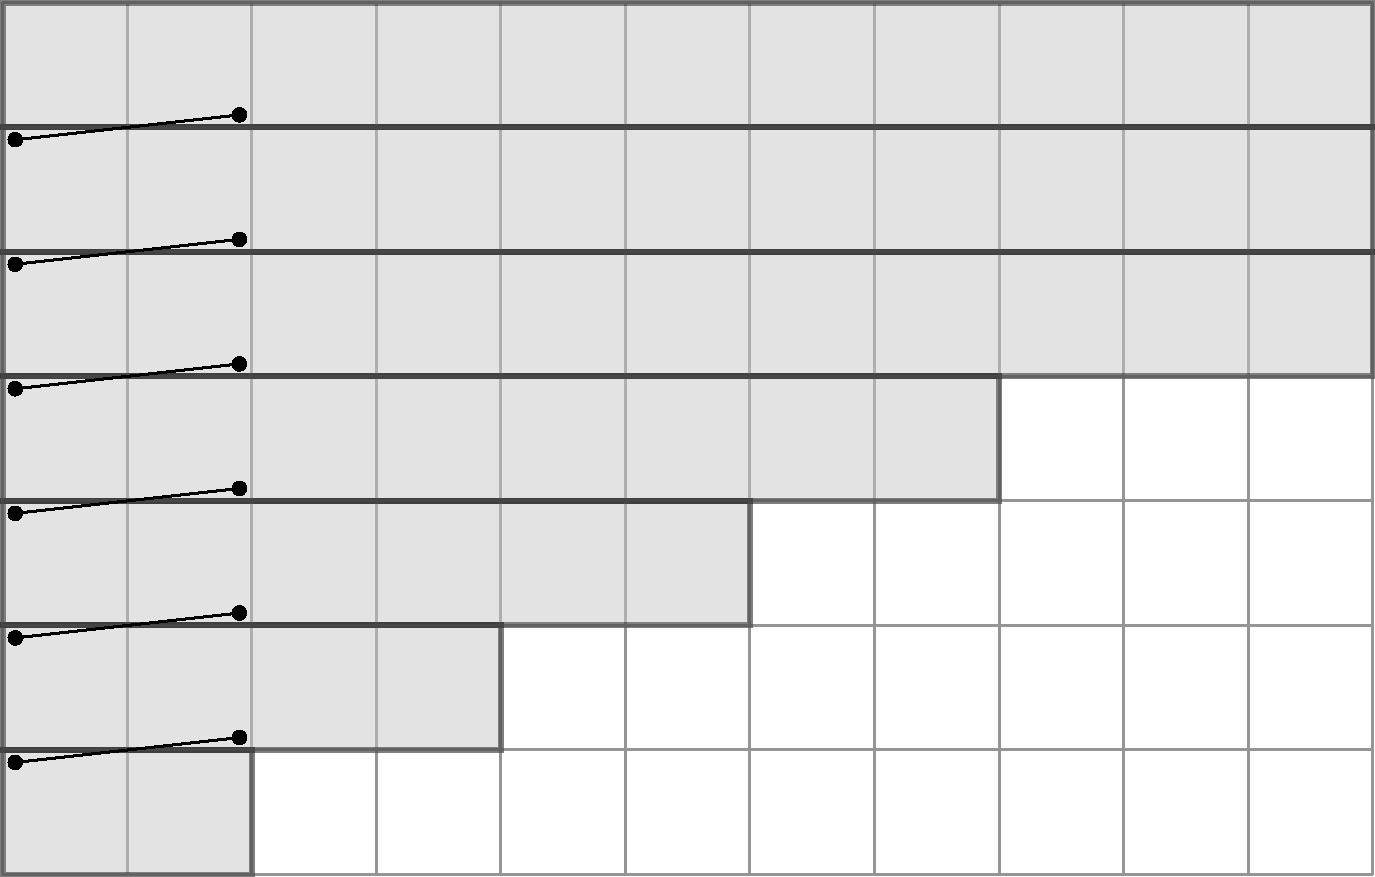
\includegraphics[width=0.5\textwidth]{WPP.jpg}
	\caption{Aaltorintamarinnakkaisen laskennan eteneminen}
	\label{fig:wpp}
\end{figure}

Aaltorintamarinnakkaisuuden riippuvuudet tarkoittavat sitä, että
laskentayksiköitä voi olla käytössä samaan aikaan ruutujen rivien verran.
Riippuvuuksista seuraa myös se, että laskentayksiköt eivät voi aloittaa
koodausta tai dekoodausta samaan aikaan, mikä aiheuttaa rinnakkaislaskennan
tehottomuutta erityisesti suurella määrällä laskentayksiköitä.
\citealt{chi} ehdottaa tähän ratkaisuksi päällekkäistä
aaltorintamaa (Overlapped Wavefront, OWF), jonka kantava idea on, että
laskentayksiköt voivat siirtyä laskemaan seuraavaa kuvaa saatuaan oman rivinsä
valmiiksi. Tämä asettaa rajoitukset sille, kuinka paljon liikekompensaatiota
voidaan käyttää. Kun komponentti tulee koodattavaksi, sen ennustamiseen
tarvittavat kompomentit täytyy olla jo koodattu. Aaltorintaman tapauksessa
tämä tarkoittaa ylempiä rivejä. Käytännössä täytyy rajoittaa ruutujenvälistä
pystysuuntaista liikekompensaatiota. (\citealt{chi})

\citealt{chi} esittää, että päällekkäinen aaltorintama tuottaa parhaat tulokset,
laattamenetelmä toiseksi parhaat ja tavallinen aaltorintama kolmanneksi parhaat
heidän testiympäristössään. Tulos antaa ymmärtää, että ehdotettu päällekkäinen
aaltorintama -menetelmä kannattaa ottaa huomioon HEVC-standardia kehittäessä.
Huomattavaa on myös, että menetelmät toimivat huomattavasti paremmin
rinnakkaisina kuin peräkkäisinä, sillä yhdessä säikeessä ajetut testit
tuottivat selvästi huonoimmat tulokset.

\paragraph{RVC-CAL-menetelmä}
Rinnakkaisen videokoodauksen ongelmia on käsitelty aiemmissa alaluvuissa. Tässä
alaluvussa esitellään eräs keino hyödyntää rinnakkaisuutta ja sen soveltamista
videokoodaukseen. Keino on RVC-CAL, erityisesti videokoodaukseen kehitetty
CAL-ohjelmointikielen toteutus (Cal Actor Language). CALin vahvuus on se, että
sillä on kääntäjiä monille alustoille, mukaan lukien moniydinprosessorit.
RVC-CALiin on saatavilla myös avoimen lähdekoodin toteutus (\citealt{orcc}).

CAL on korkean tason toimijakeskeinen tietovuo-ohjelmointikieli (high level
actor oriented dataflow programming language). Tietovuo-ohjelmoinnissa ohjelmat
mallinnetaan suunnattuina verkkoina, joiden solmuja kutsutaan toimijoiksi.
Toimijat kuvaavat mielivaltaisen monimutkaisia laskutoimituksia ja toimijoiden
väliset kaaret tiedon liikkumista toimijoiden välillä. Liikkuva tieto
abstrahoidaan merkeiksi (token). Toimijat toistuvasti ottavat sisääntulevista kaarista
merkkejä, suorittavat laskutoimituksensa ja tuottaa merkkejä ulospäin
meneviin kaariin. Kuvan \ref{fig:dataflow} tietovuokaaviossa on viisi toimijaa,
A, B, C, D ja E. Kunkin kaaren lähtöpuolella kerrotaan, kuinka monta merkkiä
kyseiseen kaareen tuotetaan ja päättymispuolella kuinka monta merkkiä kyseinen
toimija ottaa vastaan. (\citealt{rvc})

\begin{figure}[ht]
	\centering
	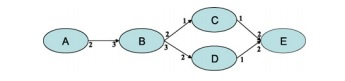
\includegraphics[width=0.5\textwidth]{dataflow.jpg}
	\caption{Yksinkertainen esimerkki tietovuokaaviosta}
	\label{fig:dataflow}
\end{figure}

Tietovuomalli perusmuodossaan ei määrää mitään aikarajoitteita toimijoiden
laskennalle. CALissa jokainen toimija on itsenäinen komponentti eivätkä muut
toimijat voi vaikuttaa sen tilaan (muuten kuin merkkejä lähettämällä). CALin
toimijat on määritelty niiden toimintojen (action) perusteella. Jokainen
toiminto määrittää miten toimijan sisäinen tila muuttuu. Toimintoja
suoritetaan (fire) riippuen merkkien sisältämästä datasta tai toimijan
sisäisistä tiedoista. Toiminnot suoritetaan peräkkäin, mutta missä toimijoiden
suoritusjärjestystä ei ole määrätty. Ominaisuuksiensa johdosta CAL sopii hyvin 
kuvaamaan rinnakkaisia järjestelmiä ja rinnakkaisia algoritmeja. (\citealt{rvc})

RVC (Reconficurable Video Coding) on MPEG-ryhmän (Moving Picture Experts
Group) kehittämä standardi rinnakkaisten videokoodausmenetelmien suunnitteluun.
Standardin tavoitteena on olla yhtenäinen, korkean tason suunnittelutyökalu.
Se määrittelee laskentayksiköt toiminnallisiksi yksiköiksi (functional unit)
ja toiminnallisten yksiköiden väliset yhteydet laskentayksiköiden välisiksi
datapoluiksi. Nämä vuorostaan kuvautuvat CALin toimijoiksi ja kuvaajien
kaariksi. CALin käyttö väliesityksenä mahdollistaa kääntämisen monenlaisille
alustoille ja jopa suoran syntetisoinnin laitteistoksi. (\citealt{rvc})

\subsubsection{Videodatan riippuvuuksien ja synkronoinnin tarpeen vähentäminen}

Videodatan riippuvuudet aiheuttavat sen, että rinnakkaistaminen on vaikeaa tai
että suurin osa rinnakkaislaskennasta kulutetaan synkronointiin eli käytännössä
tyhjäkäyntiin. Tässä aliluvussa esitellään kaksi lähestymistapaa, joilla
riippuvuuksien määrää ja niistä seuraavia ylimääräisiä kustannuksia on pyritty
vähentämään. Edellisessä aliluvussa esitellyt aaltorintamamenetelmät ja
laattamenetelmä sopisivat tähänkin lukuun, mutta seuraavassa esitettyjä
menetelmiä ei ole ehdotettu minkään standardin osaksi.

Aaltorintamamenetelmää muistuttava rinnakkaisuutta vähentävä keino on riveittäin
suoritettava koodaus (Line-By-Line Coding, LBLC). Aaltorintaman tavoin
rivikoodaus käsittelee videodatan ruutujen rivejä. Laskentayksiköille jaetaan
kuitenkin rivien sisään rivien osia. Näin rivi koodataan rinnakkaisesti ja
koodattua riviä voidaan käyttää seuraavan rivin ennustamiseen. Rikottu
riippuvuus on siis rivien vierekkäisten osien välinen. Synkronoinnin tarvetta
on vähennetty staattisella aikataulutuksella. Saman rivin osat jaetaan eri
laskentayksiköille ja eri rivien vastaavan osat samoille laskentayksiköille.
(\citealt{xu})

Esitellyt menetelmät videokoodauksen rinnakkaistamiseen ovat keskittyneet
videodatan rinnakkaisuuden rikkomiseen. On ehdotettu myös ennustamisen
tehokkaampaa rinnakkaistamista ja näin synkronoinnin huomattavaa vähenemistä.
\citealt{pieters} esittää ennustamiseen tehokkaasti rinnakkaistuvan
rekursiiviseen kaksinkertaistamiseen (recursive doubling) perustuvaa
etuliitesummaa (prefix sum) (\citealt{blelloch}). Menetelmä saa syötteekseen
perusennustuksen sekä jäännösarvot, joiden avulla näytteiden arvot on
tallennettu, kuten normaalissakin ennustamisessa. Etuliitesumma lasketaan
rinnakkaisilla laskentayksiköillä, eikä edellisten näytteiden koodausta
tarvitse odottaa. Etuliitesumma etenee puumaisesti, minkä johdosta siinä on
korkeintaan logaritminen määrä synkronointipisteitä näytteiden määrään nähden.
Kuva \ref{fig:prefix_sum} esittelee etuliitesumman etenemisen. Puun tasot ovat
mahdollisia synkronointipisteitä. (\citealt{pieters})

\begin{figure}[ht]
	\centering
	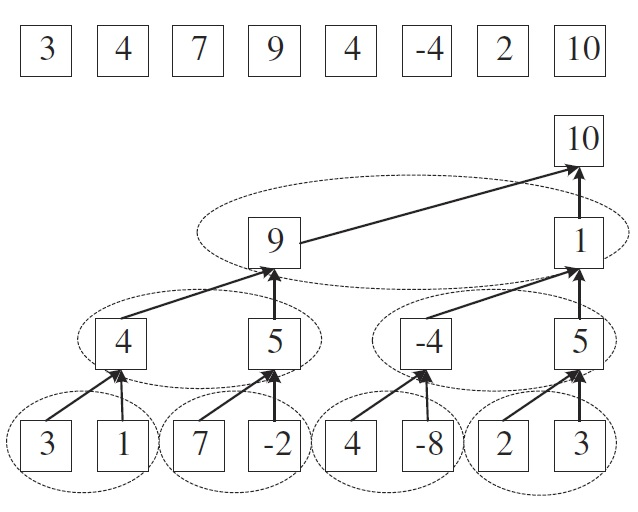
\includegraphics[width=0.5\textwidth]{prefix_sum.jpg}
	\caption{Etuliitesumma johtaa näytteen arvot jäännösarvoista}
	\label{fig:prefix_sum}
\end{figure}

Molemmat tässä kappaleessa esitellyt videokoodauksen rinnakkaistamismetodit
ovat osoittautuneet testeissä tehokkaiksi. Rivikoodaus nopeuttaa videokoodausta
lähes lineaarisesti laskentayksiköiden määrään nähden. Parhaiten se toimii
häviöttömillä ja lähes häviöttömillä koodausmenetelmillä, mikä on sopivaa,
sillä sellaiset menetelmät tarvitsevat tehokkuutta ollakseen käytännöllisiä.
(\citealt{xu}) Paremmin rinnakkaistuvat ennustaminen nopeutti H.264-standardilla
enkoodatun videon dekoodaamista 2.2-7.9 kertaisesti aaltorintamamenetelmään
verrattuna sekä 2.2 kertaista nopeutusta normaaliin ennustamiseen 2160p
-tarkkuuksisella videolla. (\citealt{pieters})

\subsubsection{Optimointi}

Uusien menetelmien kehittämisen lisäksi voidaan rinnakkaisuutta tuoda
olemassa oleviin menetelmiin niitä muuttamatta. Tällöin on tärkeää löytää
kulloinkin ratkaistavissa olevaan ongelmaan sopiva rinnakkainen lähestymistapa.
Aiemmin esiteltyjä teorioita rinnakkaisuuden mittaamisesta voidaan käyttää
erilaisten ratkaisujen analysointiin, mutta todelliset tulokset saadaan
vasta käytännön testeillä. (\citealt{li})

\citealt{li} on tutkinut H.264-standardin mukaisen videokoodauksen optimointia
rinnakkaiseen järjestelmään. Tutkimus ei esitä uusia algoritmeja
videokoodauksen ongelmien ratkaisemiseen vaan tutkii erilaisia
rinnakkaislaskentaan vaikuttavia parametreja, kuten laskentayksiköiden määrää
ja konekielisen tason optimoinnin hyödyntämistä. Suurin haitta
rinnakkaislaskennan tehokkuudelle tutkimuksessa oli laskentayksiköiden välisen
viestinnän hitaus. (\citealt{li})

Tutkimuksen tulokset osoittavat, että eräänlainen raaka rinnakkaistaminen
tehostaa videokoodausta hieman. Koska H.264 ei ole suunniteltu rinnakkaiseksi,
sen rinnakkainen tehonlisäys ei kasva lineaarisesti laskentayksiköiden määrää
kasvattaessa. Samoin yksittäisen laskentayksikön tehokkuus laskee huomattavasi
laskentayksiköiden määrää lisätessä erityisesti hitaammilla
tietoliikenneyhteyksillä. Paras tulos saavutettiin esijakamalla koodattava
videodata laskentayksiköille, jolloin sen siirtämien ei enää aiheuttanut
pullonkaulaa. Reaaliaikaiseen koodaukseen tämä ei
kuitenkaan sovi. (\citealt{li})

\subsubsection{Rinnakkaislaskennan tuomat hyödyt suorituskykyyn}

Videodataa esittelevässä luvussa esiteltiin lyhyesti erilaisia mittareita videodatan
laadulle ja videokookauksen laadulle. Taulukkoon \ref{tab:results}
erilaisten rinnakkaisten videokoodausmenetelmien tuomia hyötyjä
videokoodaukseen.
\begin{longtable}{| p{\linewidth/4} | p{\linewidth/4}| p{\linewidth/4}| p{\linewidth/4}|}

	\caption{Empiirisiä tuloksia videokoodauksen rinnakkaistamisesta}
	\label{tab:results}\\
	\hline
	Menetelmä & Mitattu suure & Saavutettu hyöty & Lähde \\
	\hline\hline
	Optimointi & Koodausnopeus & Viestikapasiteetin riittäessä lineaarinen laskentatehon kasvu laskentayksiköihin nähden &
			\citealt{li} \\
	\hline
	Rinnakkainen ennustaminen & Dekoodausnopeus &
			18.3-21.5 kertainen nopeus verrattuna aaltorintamarinnakkaisuuteen & \citealt{pieters} \\
	\hline
	Rinnakkaisuuksien rikkominen & Pakkaussuhde & Parhaimmillaan 14\% parempi pakkaussuhde verrattuna
			peräkkäiseen implementaatioon & \citealt{xu} \\
	\hline
	Rinnakkaisuuksien rikkominen & Skaalautuvuus & Lähes lineaarinen skaalautuvuus laskentayksiköiden määrään nähden &
			\citealt{xu} \\
	\hline
	Rinnakkaisuuksien rikkominen & PSNR & Korkeampi PSNR kuin peräkkäisellä menetelmällä erityisesti korkealaatuisessa videossa &
			\citealt{xu} \\
	\hline 
\end{longtable}
\subsection{Erilaiset kiihdytysalustat}

Yksi rinnakkaislaskennan haasteista on siinä, että rinnakkaiset järjestelmät
ovat hyvin erilaisia ja yhteisiä tekniikoita ja toteutuksia niille on vaikea
löytää. Tässä aliluvussa käsitellään muutamia erilaisia kiihdytysalustoja ja
niiden sopivuutta rinnakkaiseen videokoodaukseen.

Kaikenlaiset tietokoneet aina älypuhelimista tehokkaisiin palvelimiin alkavat
olla nykypäivänä moniydinprosessoreilla varustettuja (\citealt{choi}). Tämän
johdosta tätä kiihdytysalustaa voidaankin pitää tärkeänä erityisesti
multimediasovelluksille, joissa videokoodaus on yleinen ja tärkeä operaatio.
Esitellyistä tutkimuksista \citealt{chi} käytti kiihdytysalustanaan 12-ytimistä
prosessoria, kun taas \citealt{li} käytti klusteria moniytimisiä prosessoreita.
Esitetyt tulokset osoittavat, että videokoodaus voidaan onnistuneesti
rinnakkaistaa moniydinprosessoreille, mikä ennustaa hyvää tulevaisuuden
rinnakkaisille videokoodaustoteutuksille kuluttajatason tietokoneissa.

Klusteri tarkoittaa useampaa yhteen liitettyä tietokonetta, jotka on valjastettu
suorittamaan samaa tehtävää. Klusterit ovat tyypillisiä tieteelliselle ja
todella vaativalle laskennalle, joka vaatii yksittäisiä koneita suuremman 
laskentatehon. Esitellyistä tutkimuksista \citealt{li} esitteli kaksi erilaista
klusteria, toisen Windows-käyttöjärjestelmän PC:illä ja toisen
Linux-käyttöjärjestelmällä toimivilla koneilla. Klusterit tuovat 
rinnakkaislaskentaan omat haasteensa, kuten klusterin laskentayksiköiden
heterogeenisyyden, laskentayksiköiden välisen viestinnän ja esimerkiksi
klusterin hinnan. Multimedian toistamiseen klusterit ovat liian tehokkaita,
mutta esimerkiksi konenäköön tai muihin tieteellisiin sovelluksiin klustereista
ja rinnakkaisesta videokoodauksesta voi olla hyötyä.

Grafiikkaprosessorit ovat nykypäivänä käytännössä kaikista
kuluttajatietokoneista löytyviä prosessoreita, jotka ovat erikoistuneet
grafiikan piirtämiseen näyttölaitteille. Rinnakkaiseksi kiihdytysalustaksi
grafiikkaprosessorit sopivat niiden rinnakkaisen luonteen puolesta.
Nykyaikaisissa grafiikkaprosessoreissa on satoja laskentayksiköitä, joiden
kellotaajuus ei ole suuri, mutta riittävä nopeaan rinnakkaiseen laskentaan.
Esitellyistä tutkimuksista \citealt{pieters} käytti kiihdytysalustanaan
grafiikkaprosessoria.

Grafiikkaprosessorit sopivat hyvin videokoodauksen
rinnakkaislaskenta-alustoiksi, mikä on luontevaa, piirretäänhän dekoodattu
videokuva näyttölaitteelle. Joissain uusissa näytönohjaimissa on
sisäänrakennettuna tuki ja valmiit ohjelmistoratkaisut joidenkin videokoodausstandardien dekoodaamista
varten, joten omia ratkaisuja tätä varten ei välttämättä edes tarvitse tehdä (\citealt{nvidia}).

\section{Yhteenveto}
\label{chap:conclusion}

Rinnakkaiset videokoodausratkaisut ovat tulevaisuudessa välttämättömiä
videolaadun parantuessa ja rinnakkaisten laskentayksiköiden yleistyessä.
Tässä työssä esiteltiin videokoodauksen ja rinnakkaislaskennan perusteita
ongelmineen ja mahdollisuuksineen sekä videokoodauksen ja rinnakkaislaskennan
yhdistämistä. Mahdollisuuksistaan huolimatta rinnakkaislaskennalla on
haasteensa, joihin ei ole vielä yhtenäisiä ratkaisuja. Olemassa olevia
videokoodausmenetelmiä ei ole kehitetty rinnakkaislaskentaa silmällä pitäen,
joten niiden rinnakkaistaminen on erityisen vaikeaa.

Ongelmista huolimatta rinnakaislaskennasta on tutkimusten mukaan hyötyä
videokoodaukselle. Rinnakkaislaskenta nopeuttaa videokoodausta ja paikoitellen
parantaa jopa pakkaussuhdetta. Jotta rinnakkaiset ratkaisut videokoodauksen
saralla yleistyisivät, on ne otettava huomioon uusia standardeja
määriteltäessä. Määrittelyjä vaikeuttaa rinnakkaisten kiihdytysalustojen
monenkirjavuus. Askelia oikeaan suuntaan on otettu, sillä uusissa
videokoodausstandardeissa rinnakkaisuus on otettu huomioon jo
suunnitteluvaiheessa ja joissain uusissa grafiikkaprosessoreissa on
sisäänrakennettuna videodekooderi.

Tässä työssä keskityttiin videokoodauksen ja rinnakkaislaskennan perusteisiin
sekä esiteltiin joitakin ratkaisuja rinnakkaiseen videokoodaukseen keskittyen
näkyvään laskentatehon kasvuun. Videokoodauksen, rinnakkaislaskennan ja
rinnakkaisen videokoodauksen saralla tehdään aktiivista tutkimusta. Esimerkiksi
varsinainen rinnakkaislaskennan tutkimus on vahasti kääntäjien ja
käyttöjärjestelmien tutkimusta, joihin ei tässä työssä syvennytty lainkaan.
Rinnakkaislaskennan laitteistojen ja ohjelmistojen tutkimus on käytännön
sovelluksien kannalta tärkeää, mutta yksityiskohdat jätettiin tämän työn ulkopuolelle.
Työ toimii johdantona rinnakkaiseen videokoodaukseen ja ohjaa syvällisemmän
tutkimuksen pariin.

Jatkotutkimuksena olisi tärkeää selvittää, millainen rinnakkainen
lähestymistapa videokoodaukselle on helpointa toteuttaa niin, että se
palvelee mahdollisimman monia kiihdytysalustoja. RVC-CAL-menetelmän esittämä
työkalu, joka mahdollistaa rinnakkaisen koodekin kääntämisen monenlaisille
alustoille on mielenkiintoinen ja tärkeä sovellus. 

% --------------------------------------------------------------------

